\section{Ingestione e preparazione dei dati}\label{sec:ingestione}

La qualità delle risposte di un sistema RAG è limitata dalla qualità dei frammenti che il recupero può restituire:
un'informazione persa, spezzata o deformata durante la preparazione dei documenti non può essere recuperata in
seguito, per quanto accurati siano i passi successivi. Questa sezione descrive come i documenti vengono
acquisiti, convertiti in un formato uniforme, ripuliti e suddivisi in frammenti corredati di metadati. Il percorso,
riassunto nella Figura~\ref{fig:pipeline-ingestione}, è affidato ai componenti Ingestion e Chunking
(Sezione~\ref{sec:panoramica}).

\begin{figure}[H]
  \centering
  \begin{tikzpicture}[
      stage/.style={draw, thick, rounded corners=3pt, fill=blue!7, align=center, text width=1.95cm,
                   minimum height=1.05cm, font=\scriptsize\bfseries},
      res/.style={align=center, text width=2.15cm, font=\scriptsize, text=black!70, anchor=north},
      arr/.style={-{Stealth[length=2mm]}, thick, black!70},
      grp/.style={draw=gray, dashed, rounded corners=4pt, inner sep=2mm},
      grplabel/.style={font=\scriptsize\itshape, text=gray!70!black, anchor=south west},
    ]
    \node[stage] (crawl) at (0,0) {Acquisizione delle pagine web};
    \node[stage] (pre) at (2.6,0) {Pulizia dell'HTML};
    \node[stage] (conv) at (5.2,0) {Conversione (Docling)};
    \node[stage] (norm) at (7.8,0) {Normalizza\-zione};
    \node[stage] (chunk) at (10.4,0) {Chunking e metadati};
    \node[stage, fill=gray!12, dashed] (emb) at (13.0,0) {Embedding};
    \foreach \a/\b in {crawl/pre, pre/conv, conv/norm, norm/chunk, chunk/emb} \draw[arr] (\a) -- (\b);

    \node[res] at (0,-0.75) {pagine HTML e URL di provenienza};
    \node[res] at (2.6,-0.75) {solo il contenuto della pagina};
    \node[res] at (5.2,-0.75) {documento strutturato (JSON): titoli, sezioni, tabelle, immagini};
    \node[res] at (7.8,-0.75) {documento corretto dagli errori di conversione};
    \node[res] at (10.4,-0.75) {frammenti con metadati e sezioni di appartenenza};

    \begin{scope}[on background layer]
      \node[grp, fit={(crawl) (norm) (0,-3.3)}] (g1) {};
      \node[grp, fit={(chunk) (10.4,-3.3)}] (g2) {};
    \end{scope}
    \node[grplabel] at (g1.north west) {Ingestion};
    \node[grplabel] at (g2.north west) {Chunking};
    \node[font=\scriptsize\itshape, anchor=south] (pdf) at (5.2,1.05) {documenti (PDF, DOCX, PPTX, \dots)};
    \draw[arr, dashed] (pdf.south) -- (conv.north);
  \end{tikzpicture}
  \caption{Preparazione dei dati: per ogni passo, il risultato che passa al successivo. Le pagine web attraversano
  tutti i passi; gli altri documenti entrano direttamente nella conversione.}
  \label{fig:pipeline-ingestione}
\end{figure}

\subsection{Fonti dei dati}

Il sistema è pensato per indicizzare due famiglie di fonti, riassunte nella Tabella~\ref{tab:fonti}: le pagine web
pubblicate dall'ateneo e i documenti in formato file, come regolamenti, bandi, guide o materiali didattici. Per
entrambe conta, oltre al contenuto, l'\emph{ambito}: un'informazione può valere per tutti gli studenti, come le
procedure di iscrizione o le tasse, oppure solo per quelli di un corso di laurea, come il calendario della prova
finale o il regolamento del tirocinio. È questa distinzione a rendere necessario indicare, in ogni frammento, a quale
corso appartiene o se si tratta di un'informazione di ateneo, e a determinare di conseguenza come la fonte viene
acquisita e organizzata.

\begin{table}[H]
  \centering
  \small
  \begin{tabularx}{\textwidth}{@{} L{3.0cm} >{\raggedright\arraybackslash}X L{2.6cm} L{3.1cm} @{}}
    \toprule
    \textbf{Fonte} & \textbf{Esempi di contenuto} & \textbf{Formato} & \textbf{Acquisizione} \\
    \midrule
    Pagine generali di ateneo & tasse, iscrizioni, borse di studio, procedure amministrative & HTML &
      crawler, a partire dalle pagine radice delle sezioni d'interesse \\
    Siti dei corsi di laurea & piano di studi, prova finale, tirocini, scadenze, contatti & HTML &
      crawler, a partire dalla pagina radice di ogni corso \\
    Documenti di ateneo & regolamenti, bandi, guide & PDF, DOCX, PPTX e altri formati &
      file collocati nella cartella di ateneo \\
    Documenti di un corso o di un insegnamento & regolamenti del corso, slide, dispense, articoli & PDF, DOCX, PPTX
      e altri formati & file collocati nella cartella del corso e dell'insegnamento \\
    \bottomrule
  \end{tabularx}
  \caption{Tipi di fonte che il sistema può indicizzare. Le pagine dei corsi e i documenti collocati nella cartella
  di un corso ricevono l'ambito \emph{corso}; le altre fonti l'ambito \emph{ateneo}.}
  \label{tab:fonti}
\end{table}

Nel prototipo valutato in questo lavoro la base documentale comprende le pagine generali di ateneo, i siti di tre
corsi di laurea e i materiali di un insegnamento. Gli esempi riportati in questa sezione sono tratti da quel corpus.

\subsection{Acquisizione dei documenti}

Le pagine web vengono scaricate da un crawler sviluppato per il progetto. A partire da una o più pagine radice ---
ad esempio la home page del sito di un corso --- il crawler segue i collegamenti interni e scarica ogni pagina
raggiungibile, restando entro l'ambito definito dalla radice: lo stesso sito e lo stesso percorso, così che partendo
dalle pagine di un corso non si finisca su quelle di un altro.

Ogni pagina viene salvata in una cartella che riproduce il percorso del suo indirizzo: la pagina
\emph{corsi.unibo.it/laurea/Infermieristica/frequenza-delle-lezioni}, ad esempio, finisce nella cartella
\emph{laurea/Infermieristica/frequenza-delle-lezioni}. Accanto a ogni pagina viene inoltre conservato l'indirizzo esatto
da cui è stata scaricata, che diventa il collegamento mostrato allo studente tra le fonti di una risposta.

I documenti in formato file vengono invece collocati nello stesso albero di cartelle seguendo il medesimo schema:
un regolamento del corso di Infermieristica, ad esempio, va nella cartella del corso, mentre le slide di un
insegnamento vanno in una sottocartella dedicata all'insegnamento, all'interno di quella del corso; i documenti
validi per tutti gli studenti vanno nella cartella di ateneo. Questa organizzazione non è solo una comodità: la
posizione di un documento nell'albero è la fonte da cui, più avanti, vengono ricavati i metadati di ambito, di corso
e di insegnamento, così che aggiungere un documento al sistema richieda soltanto di
copiarlo nella cartella giusta.

\subsection{Pulizia delle pagine web}

Le pagine web sono progettate per essere consultate da una persona attraverso un browser, non per essere lette da
un programma, e questo introduce tre tipi di problemi nella conversione.

\paragraph{Contenuto di contorno.} Una pagina contiene molto più del suo contenuto informativo: menu di
navigazione, piè di pagina, banner dei cookie, moduli di ricerca. Ripetuti identici su ogni pagina di un sito,
questi elementi finiscono nei frammenti indicizzati, dove nella migliore delle ipotesi diluiscono il contenuto utile
e nella peggiore lo alterano, ad esempio quando il piè di pagina viene incollato all'ultimo paragrafo della pagina.
Prima della conversione, ogni pagina viene quindi ridotta al solo contenuto principale, che i siti costruiti con un
sistema di gestione dei contenuti, come quelli dell'ateneo, racchiudono in un'area dedicata della pagina, separata
da menu e piè di pagina.

\paragraph{Contenuto nascosto.} Per non sovraccaricare chi legge, molti siti mostrano le informazioni solo su
richiesta: voci che si espandono al clic, schede, note che compaiono al passaggio del mouse. Nel codice della pagina
quel contenuto è presente ma marcato come nascosto, e uno strumento di conversione, che per scelta scarta ciò che
il lettore non vede, lo perde. È una perdita silenziosa, che non produce errori ma lascia nella base documentale
pagine apparentemente complete a cui mancano proprio le informazioni di dettaglio --- contatti, passaggi di una
procedura, date --- che più spesso sono oggetto di domanda (Figura~\ref{fig:voci}). Prima della conversione,
il contenuto nascosto viene quindi reso visibile.

\begin{figure}[H]
  \centering
  \begin{tikzpicture}[
      page/.style={draw, rounded corners=2pt, fill=white, inner sep=0pt},
      acc/.style={draw, fill=blue!8, minimum width=5.2cm, minimum height=0.5cm, font=\scriptsize, anchor=west,
                  inner sep=2pt},
      body/.style={font=\scriptsize, align=left, text width=5.0cm, anchor=north west},
      arr/.style={-{Stealth[length=2mm]}, thick, black!70},
    ]
    % pagina originale
    \node[font=\footnotesize\bfseries] at (2.8,0.55) {Pagina originale};
    \draw[rounded corners=2pt, fill=white] (0,-4.6) rectangle (5.6,0.2);
    \node[acc] at (0.2,-0.25) {\textbf{+}\ \ Come immatricolarti};
    \node[acc] at (0.2,-0.85) {\textbf{+}\ \ Permesso di soggiorno e copertura sanitaria};
    \node[acc] at (0.2,-1.45) {\textbf{--}\ \ Quando sostenerla};
    \node[body] at (0.3,-1.75) {La prova di ammissione per l'a.a.\ 2026/27 si svolgerà il giorno
      \textbf{16 settembre 2026} presso il Quartiere fieristico di Bologna\dots};
    \node[font=\scriptsize\itshape, text=gray] at (2.8,-3.3) {contenuto visibile solo dopo il clic};

    \draw[arr] (5.85,-1.45) -- node[above, font=\scriptsize] {pulizia} (7.15,-1.45);

    % sezioni risultanti
    \node[font=\footnotesize\bfseries] at (10.1,0.55) {Contenuto convertito};
    \draw[rounded corners=2pt, fill=white] (7.4,-4.6) rectangle (12.8,0.2);
    \node[body, text width=5.1cm] at (7.55,0.05) {\textbf{--} Come immatricolarti: accedi a Studenti Online,
      compila la richiesta di immatricolazione\dots\\[3pt]
      \textbf{--} Permesso di soggiorno e copertura sanitaria: se vuoi iscriverti al Servizio Sanitario
      Nazionale\dots\\[3pt]
      \textbf{--} Quando sostenerla: la prova di ammissione per l'a.a.\ 2026/27 si svolgerà il giorno
      16 settembre 2026\dots};
  \end{tikzpicture}
  \caption{Voci della pagina \emph{Iscriversi al Corso} di Infermieristica. Il contenuto delle voci
  chiuse è presente nella pagina ma marcato come nascosto: senza la pulizia sarebbe stato scartato, e con esso la
  data della prova di ammissione; dopo la pulizia il contenuto di ogni voce è conservato insieme al suo titolo.}
  \label{fig:voci}
\end{figure}

\paragraph{Struttura affidata alla presentazione.} In una pagina web la struttura logica del contenuto non sempre è
espressa con gli elementi che la descrivono, come i titoli di sezione: spesso è affidata a componenti grafici, come
il titolo di una voce espandibile, che il browser mostra come un'intestazione ma che nel codice non lo è. Per lo
strumento di conversione quella struttura non esiste, e ciò che ne segue degrada i frammenti in due modi: il
contenuto di una voce viene fuso in un unico blocco, separando ad esempio un elenco dalla frase che lo introduce, e
gli elementi annidati nelle parti sbagliate si propagano, come una nota esplicativa inserita nell'intestazione di
una colonna, che diventa parte dell'intestazione e viene ripetuta su ogni riga della tabella
(Figura~\ref{fig:struttura-presentazione}). Prima della conversione,
questi componenti vengono quindi ricondotti alla struttura che rappresentano: il titolo di una voce espandibile
diventa un titolo di sezione e le note annidate vengono spostate fuori dalla struttura che altererebbero.

\begin{figure}[H]
  \centering
  \footnotesize
  \newcommand{\frag}[1]{\fbox{\parbox{0.95\linewidth}{\raggedright\scriptsize #1}}}
  \newcommand{\nota}[2]{{\color{#1}\scriptsize #2}}
  \textbf{(a) Voce espandibile con un elenco}\\[4pt]
  \begin{minipage}[t]{0.48\textwidth}
    \textit{Senza correzione: la voce resta un elemento di elenco}\\[3pt]
    \frag{\textbf{Frammento 1}\\ \ldots\ Avere l'esenzione e pagare meno tasse. Puoi ottenere un'esenzione totale o
      una riduzione delle tasse\ldots\ Hai l'esenzione totale della quota variabile e paghi solo 157,04 € se ti
      trovi in una delle seguenti condizioni: \ldots}\\[3pt]
    \frag{\textbf{Frammento 2}\\ -- l'indicatore della situazione economica del nucleo familiare è pari o
      inferiore a 27.000 €;\\ -- l'indicatore \ldots\ è pari o inferiore a 40.000 € e diventi genitore\ldots}\\[3pt]
    \nota{red!70!black}{L'elenco è separato dalla frase che lo introduce: il frammento 2 non dice a cosa servono le
      soglie.}
  \end{minipage}\hfill
  \begin{minipage}[t]{0.48\textwidth}
    \textit{Con la correzione: la voce diventa una sezione}\\[3pt]
    \frag{\textbf{Frammento}\quad\textit{Tasse ed esenzioni $>$ \ldots\ $>$ Avere l'esenzione e pagare meno
      tasse}\\[2pt] Hai l'esenzione totale della quota variabile e paghi solo 157,04 € se ti trovi in una delle
      seguenti condizioni:\\ -- l'indicatore della situazione economica del nucleo familiare è pari o inferiore a
      27.000 €;\\ -- l'indicatore \ldots\ è pari o inferiore a 40.000 € e diventi genitore\ldots}\\[3pt]
    \nota{green!40!black}{Frase introduttiva ed elenco restano nello stesso frammento, sotto il titolo della
      voce.}
  \end{minipage}

  \vspace{12pt}
  \textbf{(b) Nota a comparsa nell'intestazione di una colonna}\\[4pt]
  \begin{tikzpicture}[
      cell/.style={draw=black!40, minimum height=0.5cm, font=\scriptsize, inner sep=2pt},
      hd/.style={cell, fill=blue!8, font=\scriptsize\bfseries},
    ]
    \node[font=\scriptsize\itshape, anchor=west] at (-0.1,0.75) {Come appare nella pagina};
    \node[hd, minimum width=6.2cm, anchor=west] at (0,0) {Insegnamento};
    \node[hd, minimum width=1.4cm, anchor=west] (cfu) at (6.2,0) {CFU \textcircled{\tiny ?}};
    \foreach \y/\n/\c in {-0.5/Accertamento ed esame obiettivo infermieristico/1,
                          -1.0/Filogenesi e struttura della disciplina infermieristica/2,
                          -1.5/Metodologia infermieristica applicata/4} {
      \node[cell, minimum width=6.2cm, anchor=west, align=left, text width=6.0cm] at (0,\y) {\n};
      \node[cell, minimum width=1.4cm, anchor=west] at (6.2,\y) {\c};
    }
    \node[draw, rectangle callout, callout absolute pointer={(7.35,0.15)}, fill=yellow!12, font=\scriptsize,
          anchor=west] at (8.2,0.45) {Crediti formativi universitari};
    \node[font=\scriptsize\itshape, text=gray, anchor=west, text width=4.2cm] at (8.2,-0.6)
      {la nota compare passando con il mouse sul punto interrogativo, ma nel codice si trova dentro
      l'intestazione della colonna};
  \end{tikzpicture}\\[8pt]
  \begin{minipage}[t]{0.48\textwidth}
    \textit{Senza correzione: la nota è nell'intestazione}\\[3pt]
    \frag{Accertamento ed esame obiettivo infermieristico, \textbf{CFU ? Crediti formativi universitari} = 1\\
      Filogenesi e struttura della disciplina infermieristica, \textbf{CFU ? Crediti formativi universitari} = 2\\
      Metodologia infermieristica applicata, \textbf{CFU ? Crediti formativi universitari} = 4}\\[3pt]
    \nota{red!70!black}{La nota si ripete accanto a ogni insegnamento: in una tabella con decine di righe e note
      lunghe, il frammento si riempie di testo ripetuto.}
  \end{minipage}\hfill
  \begin{minipage}[t]{0.48\textwidth}
    \textit{Con la correzione: la nota diventa una legenda}\\[3pt]
    \frag{\texttt{| insegnamento | cfu |}\\
      \texttt{| Accertamento ed esame \ldots\ | 1 |}\\
      \texttt{| Filogenesi e struttura \ldots\ | 2 |}\\
      \texttt{| Metodologia infermieristica \ldots\ | 4 |}\\[2pt]
      Legenda -- cfu: Crediti formativi universitari}\\[3pt]
    \nota{green!40!black}{La nota compare una sola volta, subito dopo la tabella.}
  \end{minipage}
  \caption{Due effetti di una struttura affidata alla presentazione, ricostruiti in forma schematica su pagine del
  corpus del prototipo: (a) la voce \emph{Avere l'esenzione e pagare meno tasse} della pagina delle tasse di ateneo;
  (b) una tabella del piano didattico di Infermieristica (estratto: tre insegnamenti e la colonna dei crediti). A sinistra i frammenti senza la correzione, a destra
  quelli effettivamente indicizzati.}
  \label{fig:struttura-presentazione}
\end{figure}

Le regole con cui questi problemi vengono individuati dipendono da come è costruito un sito, e sono state definite
sui siti dell'ateneo; indicizzare pagine con una struttura diversa può richiederne di nuove, mentre il resto della
pipeline lavora sulla rappresentazione comune prodotta dalla conversione ed è indipendente dal sito di provenienza.

\subsection{Conversione in un formato strutturato}

Pagine web e documenti vengono convertiti con Docling~\cite{docling2024}, uno strumento open source che trasforma
documenti di formati diversi --- tra gli altri PDF, documenti Word, presentazioni PowerPoint, fogli di calcolo, pagine
HTML, Markdown e immagini --- in un'unica rappresentazione strutturata, il \emph{DoclingDocument}, salvata in formato
JSON. Il prototipo abilita PDF, DOCX, PPTX e HTML, i formati delle fonti indicizzate; gli altri formati supportati da
Docling si aggiungono estendendo l'elenco dei formati accettati dal convertitore, senza modifiche agli stadi
successivi, che lavorano sulla rappresentazione comune. A differenza di un'estrazione del solo testo, questa rappresentazione
conserva la struttura del documento: la gerarchia di titoli e sezioni, i paragrafi, gli elenchi, le tabelle con le
loro righe e colonne e le immagini, ciascuna con la propria posizione nel documento. Grazie a questa struttura,
nel passo successivo il documento può essere diviso in frammenti nei punti in cui finisce una sezione, un paragrafo
o una tabella, invece che ogni tot parole: si evita così di tagliare una frase o una tabella a metà.

La conversione si adatta al formato. Documenti Word e presentazioni contengono già una struttura esplicita ---
stili dei titoli, paragrafi, tabelle, diapositive --- che Docling legge direttamente dal file. I PDF, invece, non
contengono una struttura esplicita ma solo testo e grafica posizionati sulla pagina: Docling ne ricostruisce la
struttura con modelli di analisi del layout, che riconoscono titoli, paragrafi, tabelle e immagini; il
riconoscimento ottico dei caratteri (OCR) recupera il testo contenuto nelle immagini delle pagine, e un modello
dedicato ricostruisce righe e colonne delle tabelle. La correttezza delle tabelle è particolarmente importante nel
dominio di questo lavoro, perché è in forma di tabella che l'ateneo pubblica scadenze, importi e calendari: una
cella attribuita alla colonna sbagliata produce una data o un importo errato nella risposta.

La Figura~\ref{fig:docling-pdf} mostra il primo passaggio su un documento reale. L'analisi del layout assegna a
ogni elemento della pagina un ruolo --- titolo, paragrafo, tabella, didascalia, piè di pagina --- e ne ricava
l'ordine di lettura e la gerarchia delle sezioni; gli elementi ripetuti su ogni pagina, come il piè di pagina,
vengono riconosciuti e tenuti fuori dal testo. Il riconoscimento ottico dei caratteri (OCR) recupera invece il testo
che non esiste come tale nel file perché fa parte di un'immagine, ad esempio le etichette di un diagramma o una
pagina scansionata. Il risultato è affidabile per le singole parole, ma non per la loro disposizione: in un
diagramma il testo non segue righe ordinate, e frasi appartenenti a riquadri diversi finiscono nello stesso blocco.
Per questo, nei diagrammi, il testo dell'OCR è affiancato da una descrizione dell'immagine nel suo insieme,
discussa nel paragrafo seguente.

\begin{figure}[H]
  \centering
  \textbf{\footnotesize (a) Analisi del layout di una pagina PDF}\\[6pt]
  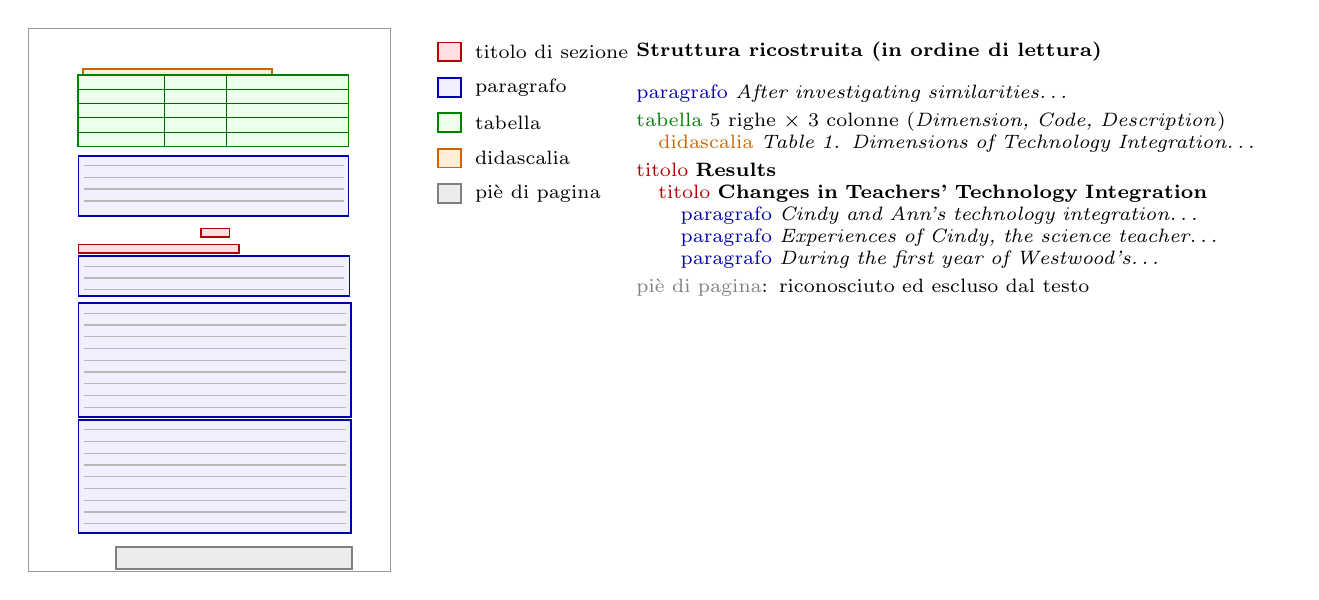
\begin{tikzpicture}[
      hd/.style={draw=red!70!black, fill=red!12, line width=0.6pt},
      tx/.style={draw=blue!70!black, fill=blue!6, line width=0.6pt},
      capt/.style={draw=orange!80!black, fill=orange!15, line width=0.6pt},
      tab/.style={draw=green!50!black, fill=green!8, line width=0.6pt},
      ft/.style={draw=gray, fill=gray!15, line width=0.6pt},
      txl/.style={gray!55, line width=0.5pt},
      tabl/.style={green!40!black, line width=0.3pt},
      leg/.style={font=\scriptsize, anchor=west},
      tree/.style={font=\scriptsize, anchor=west, align=left},
    ]
    \draw[black!40, fill=white] (0,0) rectangle (4.600,6.900);
    \draw[hd] (2.194,4.249) rectangle (2.556,4.355);
    \draw[hd] (0.639,4.046) rectangle (2.673,4.153);
    \draw[tx] (0.639,4.515) rectangle (4.068,5.281);
    \draw[txl] (0.703,5.154) -- (4.004,5.154);
    \draw[txl] (0.703,5.005) -- (4.004,5.005);
    \draw[txl] (0.703,4.856) -- (4.004,4.856);
    \draw[txl] (0.703,4.706) -- (4.004,4.706);
    \draw[tx] (0.639,3.503) rectangle (4.078,4.004);
    \draw[txl] (0.703,3.876) -- (4.014,3.876);
    \draw[txl] (0.703,3.727) -- (4.014,3.727);
    \draw[txl] (0.703,3.578) -- (4.014,3.578);
    \draw[tx] (0.639,1.959) rectangle (4.100,3.407);
    \draw[txl] (0.703,3.280) -- (4.036,3.280);
    \draw[txl] (0.703,3.131) -- (4.036,3.131);
    \draw[txl] (0.703,2.981) -- (4.036,2.981);
    \draw[txl] (0.703,2.832) -- (4.036,2.832);
    \draw[txl] (0.703,2.683) -- (4.036,2.683);
    \draw[txl] (0.703,2.534) -- (4.036,2.534);
    \draw[txl] (0.703,2.385) -- (4.036,2.385);
    \draw[txl] (0.703,2.236) -- (4.036,2.236);
    \draw[txl] (0.703,2.087) -- (4.036,2.087);
    \draw[tx] (0.639,0.490) rectangle (4.100,1.927);
    \draw[txl] (0.703,1.800) -- (4.036,1.800);
    \draw[txl] (0.703,1.650) -- (4.036,1.650);
    \draw[txl] (0.703,1.501) -- (4.036,1.501);
    \draw[txl] (0.703,1.352) -- (4.036,1.352);
    \draw[txl] (0.703,1.203) -- (4.036,1.203);
    \draw[txl] (0.703,1.054) -- (4.036,1.054);
    \draw[txl] (0.703,0.905) -- (4.036,0.905);
    \draw[txl] (0.703,0.756) -- (4.036,0.756);
    \draw[txl] (0.703,0.607) -- (4.036,0.607);
    \draw[capt] (0.692,6.314) rectangle (3.099,6.378);
    \draw[tab] (0.628,5.399) rectangle (4.068,6.304);
    \draw[ft] (1.118,0.032) rectangle (4.110,0.309);
    \draw[tabl] (0.628,6.123) -- (4.068,6.123);
    \draw[tabl] (0.628,5.942) -- (4.068,5.942);
    \draw[tabl] (0.628,5.761) -- (4.068,5.761);
    \draw[tabl] (0.628,5.580) -- (4.068,5.580);
    \draw[tabl] (1.729,5.399) -- (1.729,6.304);
    \draw[tabl] (2.520,5.399) -- (2.520,6.304);
    % legenda
    \foreach \y/\st/\t in {6.6/hd/titolo di sezione, 6.15/tx/paragrafo, 5.7/tab/tabella, 5.25/capt/didascalia,
                           4.8/ft/piè di pagina} {
      \draw[\st] (5.2,\y-0.12) rectangle (5.5,\y+0.12);
      \node[leg] at (5.55,\y) {\t};
    }
    % struttura risultante
    \node[font=\scriptsize\bfseries, anchor=west] at (7.6,6.6) {Struttura ricostruita (in ordine di lettura)};
    \node[tree, anchor=north west, text width=8.2cm] at (7.6,6.3) {%
      \textcolor{blue!70!black}{paragrafo} \emph{After investigating similarities\dots}\\[2pt]
      \textcolor{green!50!black}{tabella} 5 righe $\times$ 3 colonne (\emph{Dimension, Code, Description})\\
      \quad\textcolor{orange!80!black}{didascalia} \emph{Table 1. Dimensions of Technology Integration\dots}\\[2pt]
      \textcolor{red!70!black}{titolo} \textbf{Results}\\
      \quad\textcolor{red!70!black}{titolo} \textbf{Changes in Teachers' Technology Integration}\\
      \qquad\textcolor{blue!70!black}{paragrafo} \emph{Cindy and Ann's technology integration\dots}\\
      \qquad\textcolor{blue!70!black}{paragrafo} \emph{Experiences of Cindy, the science teacher\dots}\\
      \qquad\textcolor{blue!70!black}{paragrafo} \emph{During the first year of Westwood's\dots}\\[2pt]
      \textcolor{gray}{piè di pagina}: riconosciuto ed escluso dal testo};
  \end{tikzpicture}
  \caption{Conversione di un PDF con Docling, ridisegnata dai dati prodotti dalla conversione di un documento del
  corpus del prototipo. L'analisi del layout riconosce gli elementi della pagina, qui la pagina 9 di un
  articolo scientifico, e ne ricostruisce la gerarchia e l'ordine di lettura; il piè di pagina viene escluso dal
  testo.}
  \label{fig:docling-pdf}
\end{figure}

\paragraph{Descrizione delle immagini.} Documenti come slide e dispense contengono spesso diagrammi e schemi il
cui contenuto non è espresso nel testo circostante. Per renderlo ricercabile, ogni immagine estratta durante la
conversione viene descritta a parole da un modello linguistico capace di interpretare immagini, e la descrizione
viene inserita nel documento al posto dell'immagine stessa (Figura~\ref{fig:descrizione-immagine}). 

Il sistema usa quindi due modelli linguistici distinti: un modello multimodale, Qwen2.5-VL-7B-Instruct, che descrive
le immagini durante la conversione, e un modello solo testuale che genera le risposte. Un unico
modello multimodale per entrambi i compiti sarebbe stato più semplice da gestire, ma è stato scartato per quattro
ragioni.

\begin{itemize}
  \item \textbf{Taglia a parità di memoria.} A parità di risorse, un modello multimodale dedica una parte della
  propria capacità all'elaborazione delle immagini, e le versioni multimodali disponibili per famiglia sono meno
  numerose: per Qwen2.5 esistono in taglie da 3, 7, 32 e 72 miliardi di parametri. Con una GPU da 16~GB la più grande
  utilizzabile è quella da 7 miliardi, mentre il modello solo testuale arriva a 14 miliardi. Come discusso nella
  Sezione~\ref{sec:llm} (Figura~\ref{fig:scaling}), a parità di famiglia la taglia è il fattore che più incide sulla qualità delle risposte.
  \item \textbf{Le immagini servono una volta sola.} Il contenuto di un'immagine viene trasformato in testo durante
  la conversione e da quel momento è parte del frammento come qualunque altro paragrafo: ricercabile dal recupero e
  leggibile dal modello delle risposte. Saper interpretare le immagini è quindi necessario una volta per documento,
  al momento dell'indicizzazione, e non a ogni domanda.
  \item \textbf{Spazio nel contesto.} Passare le immagini al modello anche al momento della risposta avrebbe un costo
  diretto: ogni immagine occupa nel contesto centinaia di token, che con una finestra di 8.192 token andrebbero
  sottratti ai frammenti di testo, a vantaggio di una piccola minoranza di domande riferite a un'immagine.
  \item \textbf{Requisiti diversi.} La descrizione delle immagini è un'elaborazione fuori linea, in cui il tempo
  conta poco, mentre la generazione delle risposte deve essere rapida e sempre disponibile. Tenere separati i due
  modelli permette di avviare il modello multimodale, con una seconda istanza di vLLM, solo per la durata della
  conversione, senza fermare l'assistente mentre nuovi documenti vengono elaborati.
\end{itemize}

 Il modello
riceve un'istruzione che chiede di riportare gli elementi principali di un diagramma e le loro relazioni, il testo
leggibile e i valori di eventuali grafici. Le immagini più piccole di una soglia di area vengono ignorate, perché si tratta in
genere di loghi ed elementi decorativi; la soglia predefinita dello strumento, pensata per pagine di testo, è stata
però abbassata di dieci volte, perché su una slide un diagramma significativo occupa spesso meno del 2\% della
pagina e sarebbe stato scartato. In Docling la descrizione delle immagini fa parte dell'elaborazione dei PDF: le
immagini di documenti Word e presentazioni vengono estratte ma non descritte, e le presentazioni con contenuto
visivo rilevante conviene quindi indicizzarle esportate in PDF.

\begin{figure}[H]
  \centering
  \begin{minipage}[c]{0.42\textwidth}
    \centering
    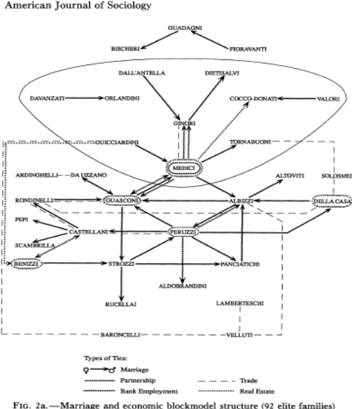
\includegraphics[width=\textwidth]{assets/famiglie_fiorentine.png}
  \end{minipage}\hfill
  \begin{minipage}[c]{0.54\textwidth}
    \footnotesize\itshape
    ``L'immagine mostra una struttura blocchi economiche-matrimoniali basata su 92 famiglie elite, come illustra la
    figura `Fig.~2a' dell'American Journal of Sociology. Il diagramma rappresenta una rete complessa che collega
    diversi nomi di famiglie aristocratiche italiane, indicando le relazioni matrimoniali e economiche tra esse.
    [\dots] Al centro si trova l'elemento `MEDICI', da cui partono numerose frecce verso altre famiglie,
    simbolizzando il dominio economico e matrimoniale della famiglia Medici sulla restante élite\dots''
  \end{minipage}
  \caption{Una figura tratta dalle slide di un insegnamento, la rete dei legami matrimoniali ed economici tra le
  famiglie dell'élite fiorentina (a sinistra), e un estratto della descrizione generata durante la conversione (a
  destra), che entra nel frammento indicizzato al posto dell'immagine. Grazie alla descrizione, una domanda come
  ``quale famiglia occupa la posizione centrale della rete?'' trova la risposta anche se il nome non compare nel
  testo della slide.}
  \label{fig:descrizione-immagine}
\end{figure}

La descrizione automatica rende ricercabile un contenuto che altrimenti non lo sarebbe, ma non è sempre fedele, e
il suo errore più insidioso non è l'omissione ma l'invenzione. La stessa descrizione della
Figura~\ref{fig:descrizione-immagine}, dopo aver colto correttamente l'insieme del diagramma, prosegue elencando
alcuni legami tra famiglie: afferma che la famiglia Valori è ``collegata direttamente'' ai Medici, mentre nel
diagramma è collegata ai Cocco-Donati; attribuisce alla famiglia Dall'Antella ``due figli sposati con membri delle
famiglie Orlandini e Coccolonati'', una famiglia che nel diagramma non compare; trasforma Altoviti in
``Aldoviti''. Sono affermazioni precise, formulate con la stessa sicurezza di quelle corrette e indistinguibili da
esse per chi legge il testo indicizzato: una domanda sui legami della famiglia Valori recupererebbe questa
descrizione, e il modello delle risposte, che si attiene fedelmente al contesto ricevuto, riporterebbe l'errore
citandone anche la fonte. Per questo il testo generato a partire dalle immagini va considerato meno affidabile di quello estratto
direttamente dai documenti, e la sua accuratezza è valutata separatamente, con domande dedicate alle immagini, nel
Capitolo~\ref{cap:validazione}.

\paragraph{La taglia del modello multimodale.} La qualità delle descrizioni dipende in misura decisiva dalla taglia
del modello che le produce. Per verificarlo, la stessa immagine della Figura~\ref{fig:descrizione-immagine} è stata
descritta anche da SmolVLM-256M, un modello multimodale da 256 milioni di parametri, circa trenta volte più piccolo
di quello adottato e abbastanza leggero da poter essere eseguito senza GPU dedicata: è il tipo di modello che si
sceglierebbe per non sottrarre risorse al resto del sistema, ed è quello provato inizialmente nel prototipo. La
Tabella~\ref{tab:taglia-vlm} riporta le descrizioni ottenute.

\begin{table}[H]
  \centering
  \footnotesize
  \begin{tabularx}{\textwidth}{@{} L{3.3cm} >{\raggedright\arraybackslash\itshape}X @{}}
    \toprule
    \textbf{Modello} & \textbf{\upshape Descrizione prodotta} \\
    \midrule
    SmolVLM-256M &
      In the image, we can see there is an object with some text and images attached to it. We can also see some
      arrows on the objects. There are trees at the top of the image. \\[3pt]
    Qwen2.5-VL-7B &
      L'immagine mostra una struttura blocchi economiche-matrimoniali basata su 92 famiglie elite [\dots] Il
      diagramma rappresenta una rete complessa che collega diversi nomi di famiglie aristocratiche italiane,
      indicando le relazioni matrimoniali e economiche tra esse. [\dots] Al centro si trova l'elemento `MEDICI',
      da cui partono numerose frecce verso altre famiglie\dots \\
    \bottomrule
  \end{tabularx}
  \caption{Descrizioni della rete delle famiglie fiorentine (Figura~\ref{fig:descrizione-immagine}) prodotte da
  due modelli multimodali di taglia diversa.}
  \label{tab:taglia-vlm}
\end{table}

Il modello piccolo fallisce producendo una descrizione generica e in parte inventata. Il modello da
7 miliardi di parametri coglie invece la natura del diagramma, la sua fonte e l'informazione principale, la
posizione centrale della famiglia Medici, che è proprio ciò che una domanda su questa immagine chiederebbe. Gli
errori di dettaglio visti sopra mostrano che la taglia maggiore riduce il problema senza eliminarlo, ma la
differenza tra le due taglie non è trascurabile: è la differenza tra una descrizione utile, da verificare, e una
inutilizzabile. È questa la ragione per cui il prototipo dedica alle descrizioni un modello multimodale di taglia
media, su una GPU propria, anziché un modello minimo; la penalità sulle ripetizioni è mantenuta anche con il modello
più grande, come ulteriore protezione contro i cicli di ripetizione.

\paragraph{Normalizzazione.} La ricostruzione della struttura di un PDF è un'operazione statistica e non è
perfetta. Alcuni dei suoi errori sono occasionali, ma altri si ripetono in modo sistematico e, poiché la
suddivisione in frammenti si basa proprio su quella struttura, si propagano a tutti i passi successivi. Dopo la
conversione, ogni documento viene quindi corretto da regole che affrontano quattro tipi di errore ricorrenti:
\begin{itemize}
  \item \textbf{titoli riconosciuti in modo errato}: un titolo classificato come testo ordinario, o diviso su due
  intestazioni, o fuso con il titolo successivo, altera la gerarchia delle sezioni, e con essa i punti in cui il
  documento viene diviso in frammenti e il percorso delle intestazioni che li accompagna. È il caso tipico dei documenti normativi, come i
  regolamenti, in cui un titolo d'articolo (``Art.~5'') viene spesso letto come un paragrafo;
  \item \textbf{elementi ripetuti di pagina}: intestazioni e piè di pagina che lo strumento non ha riconosciuto come
  tali compaiono come testo nel corpo del documento, una volta per pagina; vengono individuati perché ripetuti
  identici più volte nello stesso documento, e rimossi;
  \item \textbf{paragrafi spezzati}: un cambio di pagina o di colonna spezza un paragrafo a metà frase in due
  blocchi, che finirebbero in frammenti diversi; i blocchi consecutivi che non terminano con una punteggiatura di
  fine frase vengono ricomposti;
  \item \textbf{tabelle divise}: una tabella che prosegue sulla pagina successiva viene restituita come due tabelle
  distinte, la seconda senza intestazioni di colonna; le due parti vengono riunite, perché una tabella di scadenze o
  di importi deve restare intera per essere interpretata correttamente.
\end{itemize}

\subsection{Suddivisione in frammenti}\label{sec:chunking}

Il documento convertito viene suddiviso in frammenti con una strategia di \emph{chunking strutturale} ibrida
(Sezione~\ref{sec:rag}), offerta da Docling stesso: il documento viene diviso nei punti in cui finisce una
sezione, un paragrafo, un elenco o una tabella, e solo le parti che superano la dimensione massima vengono
ulteriormente suddivise, mentre parti consecutive troppo brevi sotto la stessa intestazione vengono riunite. La dimensione massima
di un frammento è di 512 token, contati con lo stesso tokenizzatore del modello di embedding, così che il conteggio
coincida con quello che il modello vedrà effettivamente. Il valore è stato scelto sperimentalmente: con frammenti
di 256 token la risposta si spezza più spesso tra frammenti diversi e il recupero peggiora sensibilmente, mentre
con 768 token i risultati restano equivalenti.

Ogni frammento conserva il \emph{percorso delle intestazioni} della sezione da cui proviene, ad esempio
\emph{Prova finale: modalità e scadenze $>$ SCADENZE}. Il percorso è essenziale per frammenti che, letti da soli,
sarebbero ambigui: una riga come ``Estivo: 2 giugno 2026, 19 giugno 2026\dots'' acquista significato solo sapendo
che appartiene al calendario delle scadenze della prova finale. Per questo il percorso viene incluso sia nella
rappresentazione vettoriale del frammento sia nel testo valutato dal modello di reranking. Non viene invece
introdotta alcuna sovrapposizione tra frammenti consecutivi. Quando si taglia ogni tot parole è utile ripetere
l'ultima parte di un frammento all'inizio del successivo, perché il taglio può cadere a metà di una frase; qui
invece il taglio cade sempre alla fine di una sezione, di un paragrafo o di una tabella, e il contesto più ampio di
un frammento è comunque recuperabile attraverso la sua sezione di appartenenza, come descritto più avanti.

Tre ulteriori interventi affrontano problemi ricorrenti nei contenuti amministrativi e didattici.

\begin{itemize}
  \item \textbf{Tabelle.} Scadenze, importi e calendari sono pubblicati quasi sempre in forma di tabella, ma il
  modo in cui una tabella è scritta raramente corrisponde al modo in cui viene interrogata. Le intestazioni sono
  spesso in maiuscolo e le date in forma numerica, mentre chi pone una domanda scrive ``l'appello di ottobre'' o ``il
  16 luglio'': la distanza lessicale abbassa la pertinenza che il recupero attribuisce alla tabella, proprio per le
  domande a cui risponde. Le tabelle vengono quindi riscritte nella forma delle domande usando
  date per esteso (Figura~\ref{fig:tabella-leggibile}). L'effetto è misurabile: per la domanda ``scadenza della domanda
  di laurea tardiva per l'appello di ottobre'', la pertinenza attribuita dal reranker alla tabella delle scadenze
  passa da 0,589 a 0,840.
  \item \textbf{Frammenti troppo brevi.} Un frammento di poche parole, tipicamente la frase introduttiva di una
  sezione senza altri frammenti con cui essere riunito, è poco distintivo per il recupero; i frammenti sotto i 40
  token vengono quindi accorpati al frammento adiacente.
  \item \textbf{Collegamenti.} I collegamenti ipertestuali vengono ridotti al solo testo visibile, eliminando
  l'indirizzo: un frammento riporta ``simula l'importo delle tasse'' anziché un lungo URL che non aggiunge
  significato e consuma spazio.
\end{itemize}

\begin{figure}[H]
  \centering
  \begin{minipage}{\textwidth}
    \textbf{\footnotesize Prima}\\[2pt]
    \fbox{\parbox{0.97\textwidth}{\ttfamily\scriptsize
      | **SCADENZA PRESENTAZIONE DOMANDA DI LAUREA** | **SCADENZA DOMANDA DI LAUREA TARDIVA** | **APPELLO DI LAUREA** |\\
      | - | - | - |\\
      | 04/06/2026 | 18/06/2026 | 16/07/2026 |\\
      | 19/08/2026 | 03/09/2026 | 01/10/2026 |}}\\[6pt]
    \textbf{\footnotesize Dopo}\\[2pt]
    \fbox{\parbox{0.97\textwidth}{\ttfamily\scriptsize
      | scadenza presentazione domanda di laurea | scadenza domanda di laurea tardiva | appello di laurea |\\
      | - | - | - |\\
      | 4 giugno 2026 | 18 giugno 2026 | 16 luglio 2026 |\\
      | 19 agosto 2026 | 3 settembre 2026 | 1 ottobre 2026 |}}
  \end{minipage}
  \caption{Riscrittura di una tabella delle scadenze della prova finale di Ingegneria e scienze informatiche: date per esteso, nella forma in cui compaiono
  nelle domande degli studenti. Il testo ``Dopo'' è quello effettivamente indicizzato.}
  \label{fig:tabella-leggibile}
\end{figure}

\paragraph{Sezioni e fusione gerarchica.} Oltre ai frammenti, che sono le unità effettivamente indicizzate e
confrontate con la domanda, il sistema conserva anche le \emph{sezioni} a cui appartengono: per ogni sezione divisa
in almeno due frammenti viene costruito un nodo che li raggruppa (Figura~\ref{fig:frammenti-sezioni}). Le sezioni
non vengono indicizzate, ma servono al recupero per la fusione gerarchica (Sezione~\ref{sec:rag}): quando tra i
frammenti selezionati per una domanda ne compaiono abbastanza della stessa sezione, questi vengono sostituiti dalla
sezione intera, così che il modello riceva un contesto completo e coerente invece di parti isolate.

\begin{figure}[H]
  \centering
  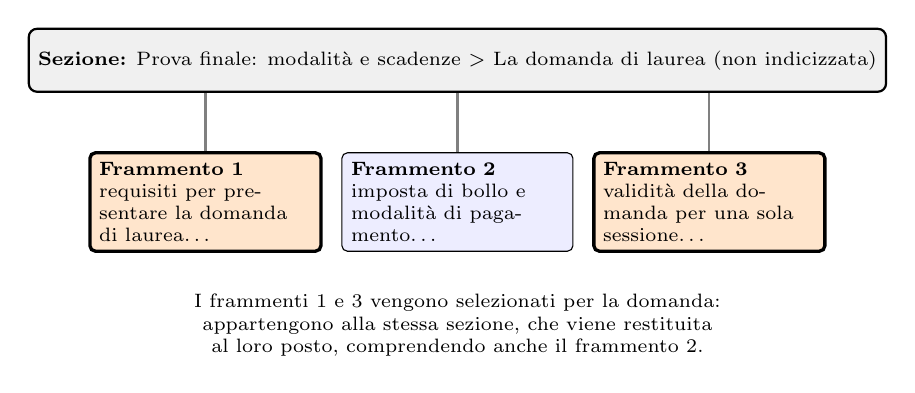
\begin{tikzpicture}[
      sec/.style={draw, thick, rounded corners=3pt, fill=gray!12, align=center, font=\scriptsize,
                  minimum width=9.2cm, minimum height=0.8cm},
      leaf/.style={draw, rounded corners=2pt, fill=blue!7, align=left, font=\scriptsize, text width=2.7cm,
                   minimum height=1.25cm},
      sel/.style={leaf, fill=orange!20, very thick},
      arr/.style={-{Stealth[length=2mm]}, thick, black!70},
    ]
    \node[sec] (s) at (0,0) {\textbf{Sezione:} Prova finale: modalità e scadenze $>$ La domanda di laurea (non
      indicizzata)};
    \node[sel] (f1) at (-3.2,-1.8) {\textbf{Frammento 1}\\ requisiti per presentare la domanda di laurea\dots};
    \node[leaf] (f2) at (0,-1.8) {\textbf{Frammento 2}\\ imposta di bollo e modalità di pagamento\dots};
    \node[sel] (f3) at (3.2,-1.8) {\textbf{Frammento 3}\\ validità della domanda per una sola sessione\dots};
    \foreach \f in {f1,f2,f3} \draw[thick, black!50] (s.south -| \f.north) -- (\f.north);
    \node[font=\scriptsize, align=center, text width=9.5cm, anchor=north] at (0,-2.85)
      {I frammenti 1 e 3 vengono selezionati per la domanda: appartengono alla stessa sezione, che viene
      restituita al loro posto, comprendendo anche il frammento 2.};
  \end{tikzpicture}
  \caption{Frammenti e sezioni. Solo i frammenti vengono indicizzati e confrontati con la domanda; le sezioni
  permettono di restituire al modello un contesto più ampio quando più frammenti della stessa sezione risultano
  pertinenti.}
  \label{fig:frammenti-sezioni}
\end{figure}

La lunghezza dei frammenti dipende dal tipo di fonte. Le sezioni delle pagine web sono in genere più brevi del
limite e restano in un unico frammento, mentre le sezioni lunghe di regolamenti, dispense e pagine più estese vengono
suddivise: nel corpus del prototipo, ad esempio, i frammenti hanno una lunghezza mediana di 117 token, ben al di
sotto del limite di 512.

\subsection{Metadati}\label{sec:metadati}

A ogni frammento viene associato un insieme di metadati, riportati nella Tabella~\ref{tab:metadati} per un
frammento del materiale del corso di Tecniche di Consulenza nella Scuola, relativo al \emph{Change Laboratory}. I
metadati di corso vengono ricavati dalla posizione del documento nell'albero delle cartelle prodotto
dall'acquisizione: per i documenti di un corso, pagine web o file, i livelli del percorso indicano il tipo di
laurea, il corso, la sezione e, per i materiali didattici, l'insegnamento; i documenti di ateneo, che seguono
un'organizzazione diversa, ricevono invece l'indicazione \emph{ateneo} e nessun corso. È su questi due campi, ambito
e corso, che si basa la gestione dei corsi: limitare la ricerca alle
pagine di ateneo e a quelle del corso dello studente, e privilegiare queste ultime.

\begin{table}[H]
  \centering
  \small
  \begin{tabularx}{\textwidth}{@{} l >{\raggedright\arraybackslash}X >{\raggedright\arraybackslash}X @{}}
    \toprule
    \textbf{Campo} & \textbf{Significato} & \textbf{Esempio} \\
    \midrule
    ambito & documento di un corso o di ateneo & corso \\
    tipo di laurea & laurea, laurea magistrale & laurea magistrale \\
    corso & corso di laurea a cui appartiene il documento & PsicologiaScolasticaComunita \\
    sezione & sezione del sito o cartella da cui proviene il documento & corsi \\
    insegnamento & insegnamento a cui si riferisce un materiale didattico & TecnicheDiConsulenzaNellaScuola \\
    intestazioni & percorso dei titoli della sezione & Change Laboratory (Change Lab) \\
    URL di provenienza & indirizzo della pagina web originale, mostrato tra le fonti &
      --- (materiale didattico caricato come file, non pagina web) \\
    identificativo & ricavato in modo stabile dal percorso del documento & 3e53833e-ffc7-5e84-ab82-9a13a6776148 \\
    impronta del contenuto & firma del file originale, per riconoscerne le modifiche & 8e837f4622a5b4e2 \\
    immagini & immagini associate al frammento, se presenti & --- (nessuna in questo frammento) \\
    \bottomrule
  \end{tabularx}
  \caption{Metadati associati a ogni frammento, con i valori reali di un frammento del materiale didattico del corso
  di Tecniche di Consulenza nella Scuola, sul metodo del \emph{Change Laboratory}: a differenza di una pagina web
  crawlata, un materiale didattico caricato come file non ha un URL di provenienza, ma valorizza il campo
  insegnamento.}
  \label{tab:metadati}
\end{table}

\paragraph{Aggiornamento incrementale.} Pagine e documenti dell'ateneo cambiano nel tempo, ad esempio a ogni nuovo anno
accademico, e ripetere l'intera preparazione a ogni modifica sarebbe inutilmente costoso, soprattutto per i PDF, la cui
conversione richiede l'analisi del layout, l'OCR e la descrizione delle immagini. Ogni frammento conserva quindi
l'impronta del documento da cui proviene, calcolata sul file originale. A ogni nuova esecuzione vengono elaborati
solo i documenti nuovi e quelli la cui impronta è cambiata; per questi ultimi, i frammenti precedenti vengono prima
eliminati sia dall'archivio sia dal database vettoriale, così che la versione aggiornata li sostituisca invece di
affiancarsi a quella superata. L'identificativo di ogni documento è ricavato in modo deterministico dal suo
percorso, così che lo stesso documento mantenga lo stesso identificativo da un'esecuzione all'altra.
